\documentclass[11pt]{article}
\usepackage{gstyle}
\title{Differential Equations Week \textbf{11}}
\author{Garud Shah}
\begin{document}
    \maketitle \newpage 
    \begin{problem}[Problem 1]
        \setcounter{equation}{-1} \break
        For the differential equations:
        \begin{align}
            x' &= y \\
            y' &= -x + x^3,
        \end{align}
        \begin{enumerate}[(a)]
            \item Sketch the direction field using computer software.
            \item Find whether the solution passing through each of the following points is periodic:
            \begin{enumerate}[i.]
                \item (0.25, 0.25)
                \item (2,2)
                \item (1,0)
            \end{enumerate}
        \end{enumerate}
    \end{problem}
    \begin{solution}[Phase planes are cool! - 1a] 
        \textit{$\text{ }$ \newline Created with https://aeb019.hosted.uark.edu/pplane.html}
        \begin{center}
            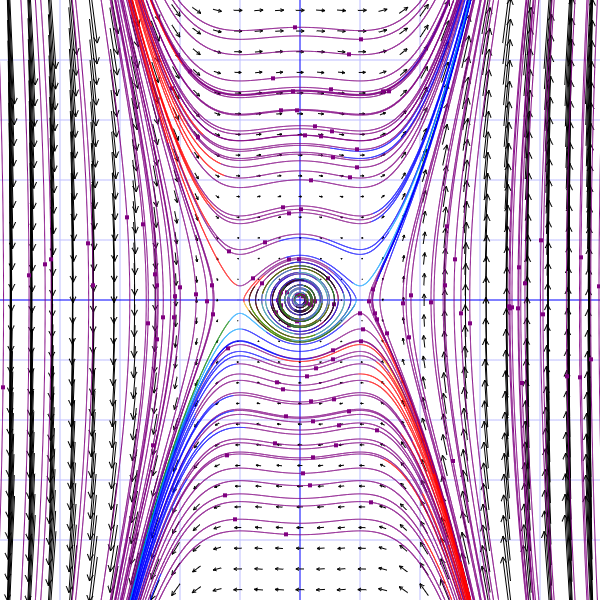
\includegraphics[scale=0.3]{1.png}
        \end{center}
        \begin{center}
            \textit{Figure 1.1: Phase plane of differential equation.}
        \end{center}
    \end{solution}
    \begin{example*}[Answers 1b]My answers are:
        \begin{enumerate}[i.]
            \item (0.25, 0.25): Why not? 
            \item (2,2): No way.
            \item (1,0): Even better: critical point, you're never leaving.
        \end{enumerate}
    \end{example*}
    \begin{problem}
        \setcounter{equation}{-1} \break
        For the differential equations
        \begin{align}
            x' &= y \\
            y' &= -x - x^3,
        \end{align}
        \begin{enumerate}[(a)]
            \item Sketch the direction field using computer software.
            \item Conjecture whether all solutions are bounded.
            \item Solve the phase plane differential equation.
        \end{enumerate}
    \end{problem}
    \begin{solution}[Phase planes are cool! - 2a] 
        \textit{$\text{ }$ \newline Created with https://aeb019.hosted.uark.edu/pplane.html}
        \begin{center}
            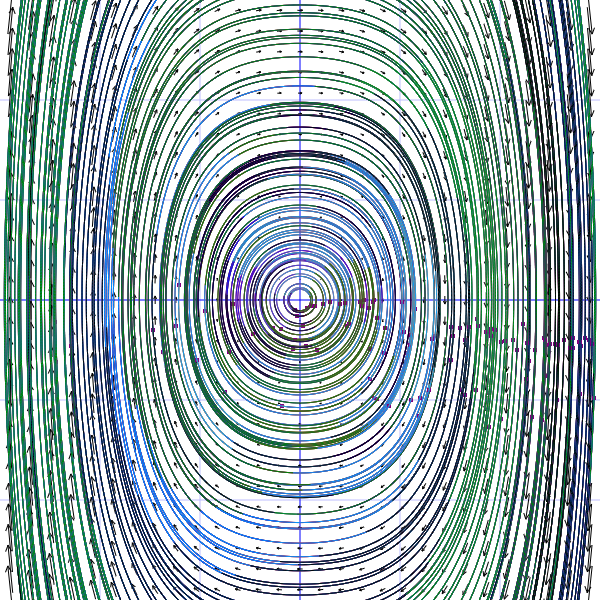
\includegraphics[scale=0.3]{2.png}
        \end{center}
        \begin{center}
            \textit{Figure 2.1: Phase plane of differential equation.}
        \end{center}
    \end{solution}
    \begin{solution}[Answer 2b]
        Why not? Looks like it.
    \end{solution}
    \begin{solution}[Solution 2c]
        We have:
        \begin{align}
            \dfrac{dy}{dx} &= \dfrac{-x-x^3}{y} \\
            y^2 &= C-x^2- \dfrac{x^4}{2} \\
            y &= \sqrt{ C-x^2- \dfrac{x^4}{2}}.
        \end{align} 
        Also this is literally a Duffing Equation in disguise so of course it's periodic.
    \end{solution}
    \newpage
    \begin{problem}
        \setcounter{equation}{-1} \break
        For the differential equations:
        \begin{align}
            x' &= (x-1)(y-1) \\
            y' &= y(y-1),
        \end{align}
        \begin{enumerate}[(a)]
            \item Construct the phase plane analysis by hand, and graph, without using computer software, the asymptotic behaviour of trajectories (as $t \rightarrow \infty$).
            \item Sketch the direction field using computer software.
            \item Solve the differential equation.
        \end{enumerate}
    \end{problem}
    \begin{solution}
        \textit{$\text{ }$ \newline}
        \begin{center}
            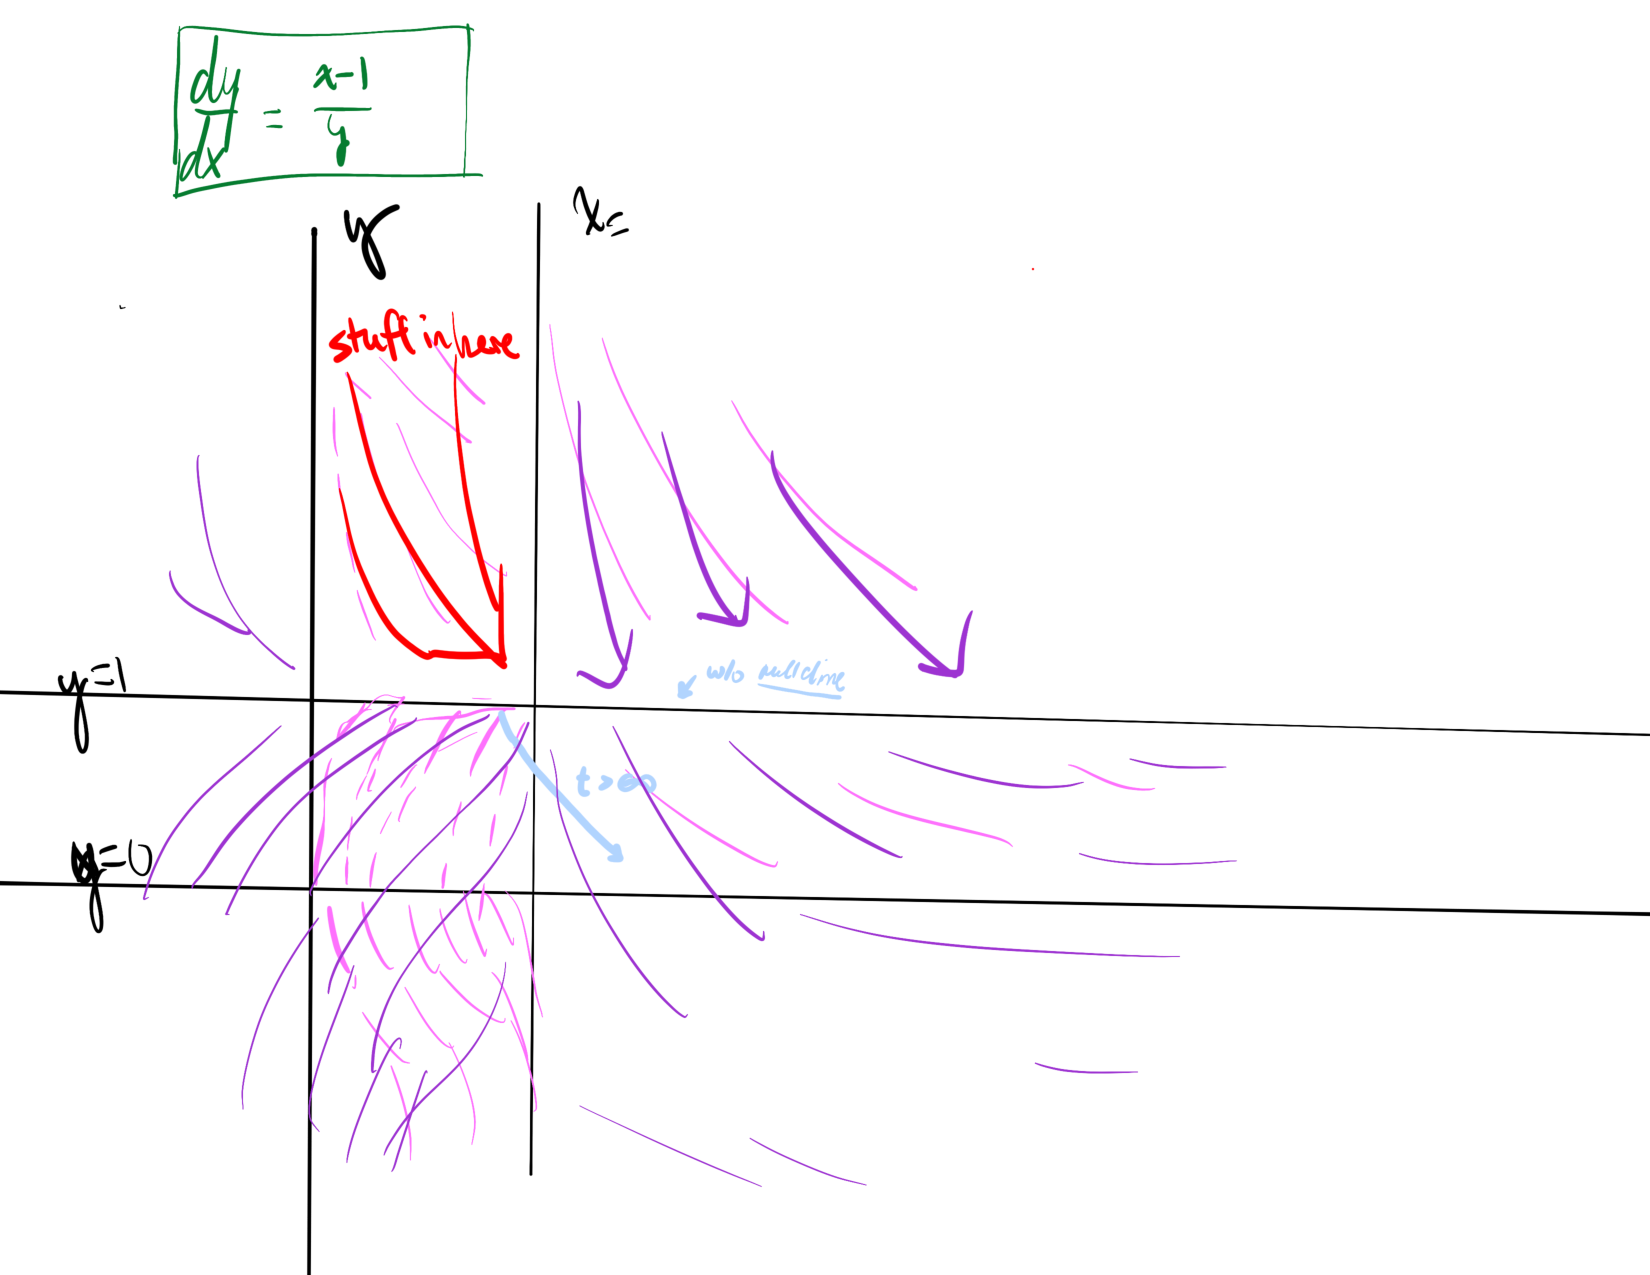
\includegraphics[scale=0.3]{3.pdf}
        \end{center}
        \begin{center}
            \textit{Figure 3.1: Hand-drawn phase plane of differential equation.}
        \end{center}
    \end{solution}
    \begin{solution}\textit{$\text{ }$ \newline Created with https://aeb019.hosted.uark.edu/pplane.html}
        \begin{center}
            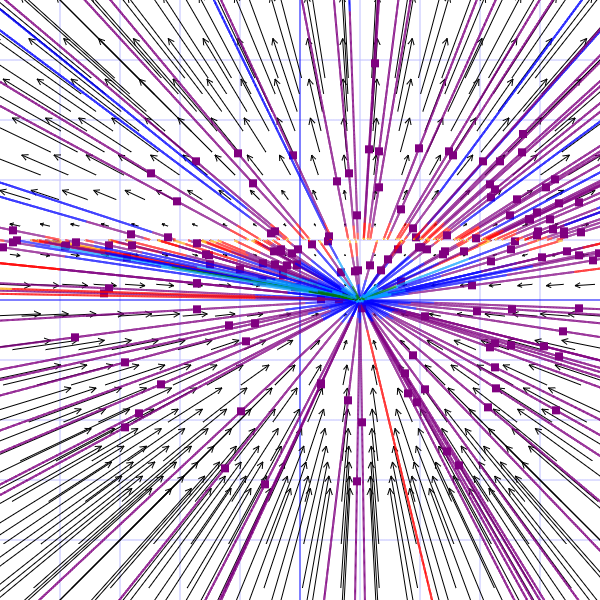
\includegraphics[scale=0.3]{3.png}
        \end{center}
        \begin{center}
            \textit{Figure 3.1: Phase plane of differential equation.}
        \end{center}
    \end{solution}
    \begin{solution}
        We solve for $y$, then $x$. \\~\\
        Note that by seperation of variables 
        \begin{align}
            y' &= y(y-1) \\
            \dfrac{y'}{y(y-1)} &= 1 \\
            \int \dfrac{dy}{y(y-1)} &= t \\
            \log \left|\dfrac{y-1}{y}\right| &= t + C \\
            \dfrac{y-1}{y} &= Ce^t \\
            y(1-Ce^t) &= -1 \\
            y &= \dfrac{1}{Ce^t-1}
        \end{align}
    \end{solution}
    \begin{problem}
        \setcounter{equation}{-1} \break
        Consider the system:
        \begin{align}
            v' &= -x+\dfrac{1}{\lambda - x} \\
            x' &= v.
        \end{align}
        \begin{enumerate}[(a)]
            \item Solve this equation in the phase plane.
            \item Find the critical points of this system. 
            \item Plot the phase plane diagrams for $\lambda=1,3$ and describe $x$ for $\lambda = 1,3$ under various initial conditions.
        \end{enumerate}
    \end{problem}
    \begin{solution}
        We note that:
        \begin{align}
            \dfrac{dv}{dx} &= \dfrac{-x+1/(\lambda -x)}{v} \\
            \dfrac{v^2}{2} &= \int -x+\dfrac{1}{\lambda - x} \, dx \\
            &= -\dfrac{x^2}{2}-\log|x-\lambda| + C.
            v^2  &= C-x^2 -\log((x-\lambda)^2) \\
            v &= \pm \sqrt{C-x^2 -\log((x-\lambda)^2)} \\
        \end{align}
    \end{solution}
    \begin{solution} \hfill
        \begin{observation}
            $v=0$ for any critical point. (obviously, bottom equation).
        \end{observation}
        Now:
        \begin{align}
            0 &= -x + \dfrac{1}{\lambda-x} \\
            x &= \dfrac{1}{\lambda - x} \\
            x^2 - \lambda x + 1 &= 0 \\
            x &= \dfrac{\lambda \pm \sqrt{\lambda^2 - 4}}{2}.
        \end{align}
        Thus to have critical points, we need $\lambda < 2$. 
    \end{solution}
    \begin{solution}\textit{$\text{ }$ \newline Created with https://aeb019.hosted.uark.edu/pplane.html}
        \begin{center}
            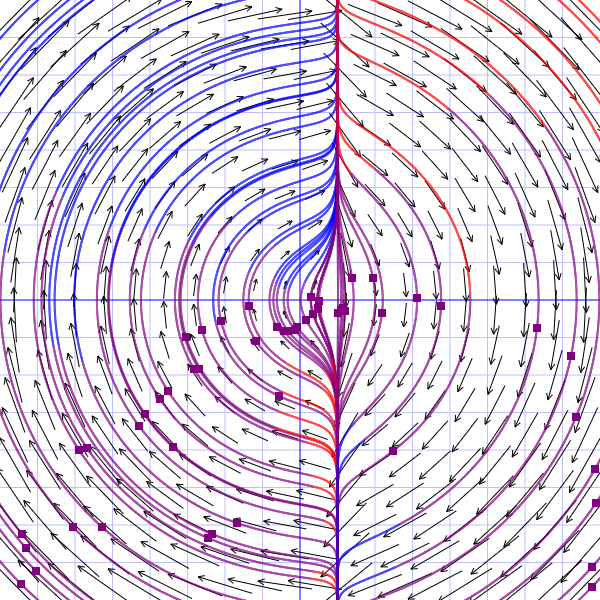
\includegraphics[scale=0.3]{41.png}
        \end{center}
        \begin{center}
            \textit{Figure 4.1: Phase plane of differential equation, $\lambda = 1$.}
        \end{center}
        It acclerates, faster and faster, until it has reached the wire.
        \begin{center}
            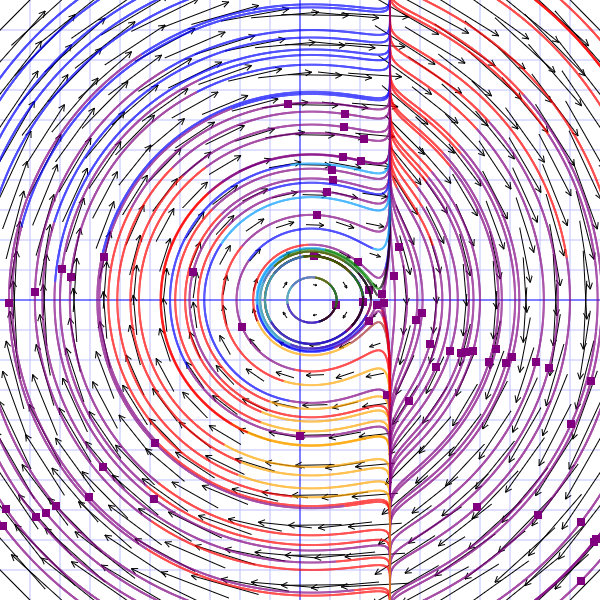
\includegraphics[scale=0.3]{43.png}
        \end{center}
        \begin{center}
            \textit{Figure 4.2: Phase plane of differential equation, $\lambda = 3$.}
        \end{center}
        It will perform behaviour as earlier, but with a bit more of a detour around the zone of stability and closed paths.
    \end{solution}
\end{document}